\chapter{Future Works}
\thispagestyle{chapterfancy}

In this chapter we will present some ideas on how to expand on the work presented in this thesis, both on the Deep Learning and the Malware Analysis aspects.

\section{Generalized Supervised Contrastive Loss}
As can be seen in Code Listing \ref{code:JSON}, Anti-Viruses (AVs) don't always agree on the label provided for a specific malware sample. However, since supervised contrastive learning (SupCon \cite{khosla2020supervised}) inherently employs label information in a binary form, during our experiments we decided to use as a ground-truth label the argmax of the possible labels. \\
A new approach could be to represent label information as a probability distribution. For example, using the AVclass labels in Code Listing \ref{code:JSON}:

\begin{lstlisting}[language=json, xrightmargin=.675\textwidth]
 "avclass_labels": {
     "ddos": 3,
     "gafgyt": 14,
     "mirai": 2
 }
\end{lstlisting}

\noindent the label vector for SupCon would be $[0,1,0]$, while, with the new approach, the new label vector would be $\left[\frac{3}{19},\frac{14}{19},\frac{2}{19}\right]\approx[0.16,0.74,0.10]$. \\
To properly take advantage of this new  label representation, a new loss function is needed: the Generalized Supervised Contrastive Loss (GenSCL \cite{kim2022generalized}). \\
Proposed by Kim \textit{et al.}, this work builds on the supervised contrastive loss but is capable of leveraging label information as a probability distribution. \\
To fully utilize the label information in the form of the probability distribution, generalized supervised contrastive aims to minimize cross-entropy between label similarity space $Y(i)\equiv\{\text{sim}(y_{i},y_{l})\}_{l\in A(i)}$ and latent similarity space $Z(i)\equiv\{P_{il}\}_{l\in A(i)}$ with respect to anchor $i$, where

\begin{equation}
\text{sim}(u,v) = \frac{u^{T}v}{\norm{u}\norm{v}} \quad\text{and}\quad P_{ij}=\frac{\exp \left(\frac{z_{i} \cdot z_{j}}{\tau}\right)}{\sum_{a\in A(i)} \exp \left(\frac{z_{i} \cdot z_{a}}{\tau}\right)} 
\end{equation}

\noindent Being $I$ the set of indices of the inputs, $z_{i}$ the embedding of the input $x_{i}$, $y_{i}$ the label of the input $x_{i}$, $\tau\in\mathbb{R}^{+}$ a scalar temperature parameter, and $A(i)\equiv I\backslash\{i\}$, the generalized supervised contrastive loss takes the following form:

\begin{equation}\label{eq:GenSCL}
    \begin{aligned} \mathcal{L}^{gen}=\sum_{i \in I} \mathcal{L}_{i}^{gen}
    & =\sum_{i \in I} \frac{1}{|A(i)|} \text{CE}(Y(i), Z(i)) \\ 
    & =\sum_{i \in I} \frac{-1}{|A(i)|} \sum_{j \in A(i)} \operatorname{sim}\left(y_{i}, y_{j}\right) \log \frac{\exp \left(\frac{z_{i} \cdot z_{j}}{\tau}\right)}{\sum_{a\in A(i)} \exp \left(\frac{z_{i} \cdot z_{a}}{\tau}\right)}
    \end{aligned}
\end{equation}

\noindent Here CE denotes cross-entropy loss. As shown in Eq. \ref{eq:GenSCL}, generalized supervised contrastive loss no longer depends on the positive contrasts set $P(i)$ which enforces the use of one-hot encoded labels, as shown in Eq. \ref{eq:SupConLoss}. Intuitively, the generalized supervised contrastive loss considers drawing positive contrasts to an anchor delicately according to label similarity, instead of pulling all positive contrasts evenly as in previous contrastive losses (Figure \ref{fig:SupConVSGenSCL}). \\

\begin{figure}[H]
    \centering
    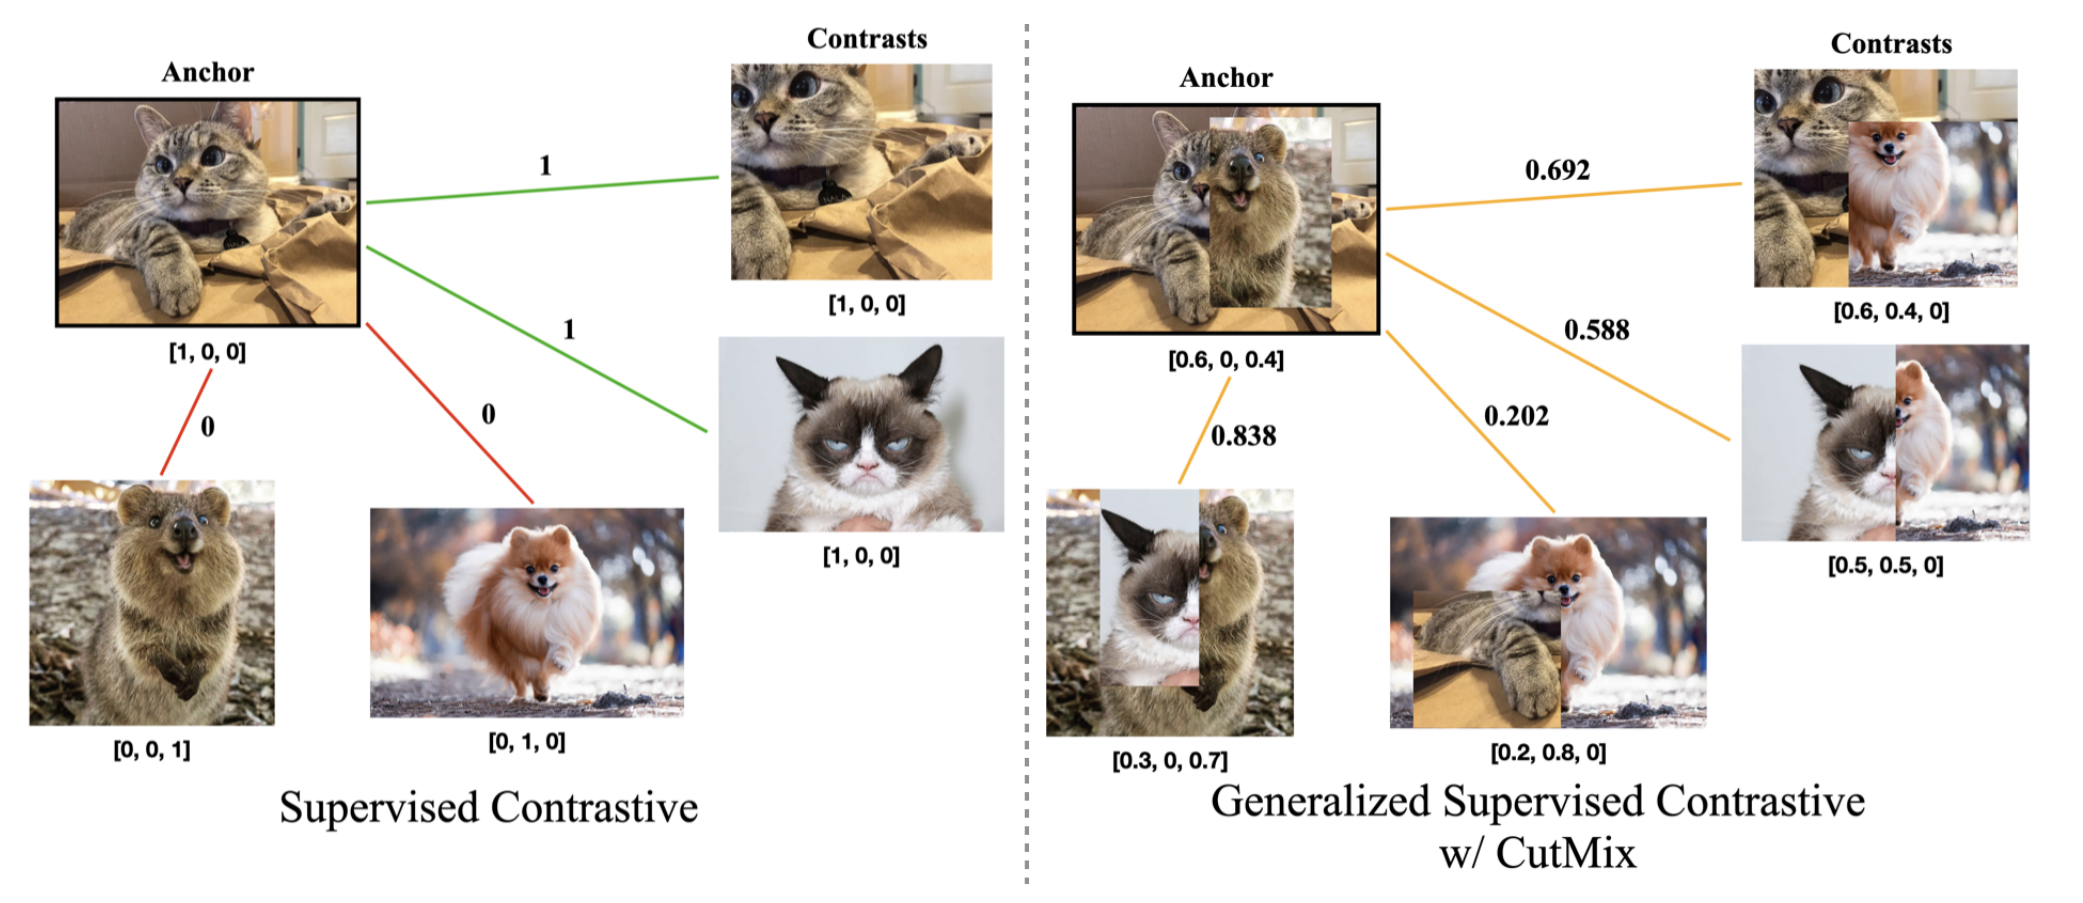
\includegraphics[width=0.9\linewidth]{Images/SupConVSGenSCL.png}
    \caption{Generalized Supervised vs. Supervised Contrastive Losses.}
    \label{fig:SupConVSGenSCL}
\end{figure}

\noindent Using this new kind of approach wouldn't probably increase performance per se, but it will create embeddings capable to better represent the malware sample from which they were generated.

\section{Symbol Extraction and Recognition}
Most Linux IoT malware classifiers and clustering rely on symbols to be able to extract information from the samples. An extensive study on Linux IoT malware has been provided by Emanuele Cozzi \cite{cozzi2020tangled}. In it, he shows that, as of 2020, over $90\%$ of Linux IoT malware samples were statically linked, and half of them were stripped, a tendency that has more that likely increased over the years. \\
Another tendency that hinders malware classification is code reuse. Since many of the most common malware families have their source code freely available online, many other families simply copy and paste their function in their own code. It can be seen in Figure \ref{fig:CodeReuse} how many functions are in common between the top-10 malware families, as reported by Cozzi \cite{cozzi2020tangled}.

\begin{figure}[H]
    \centering
    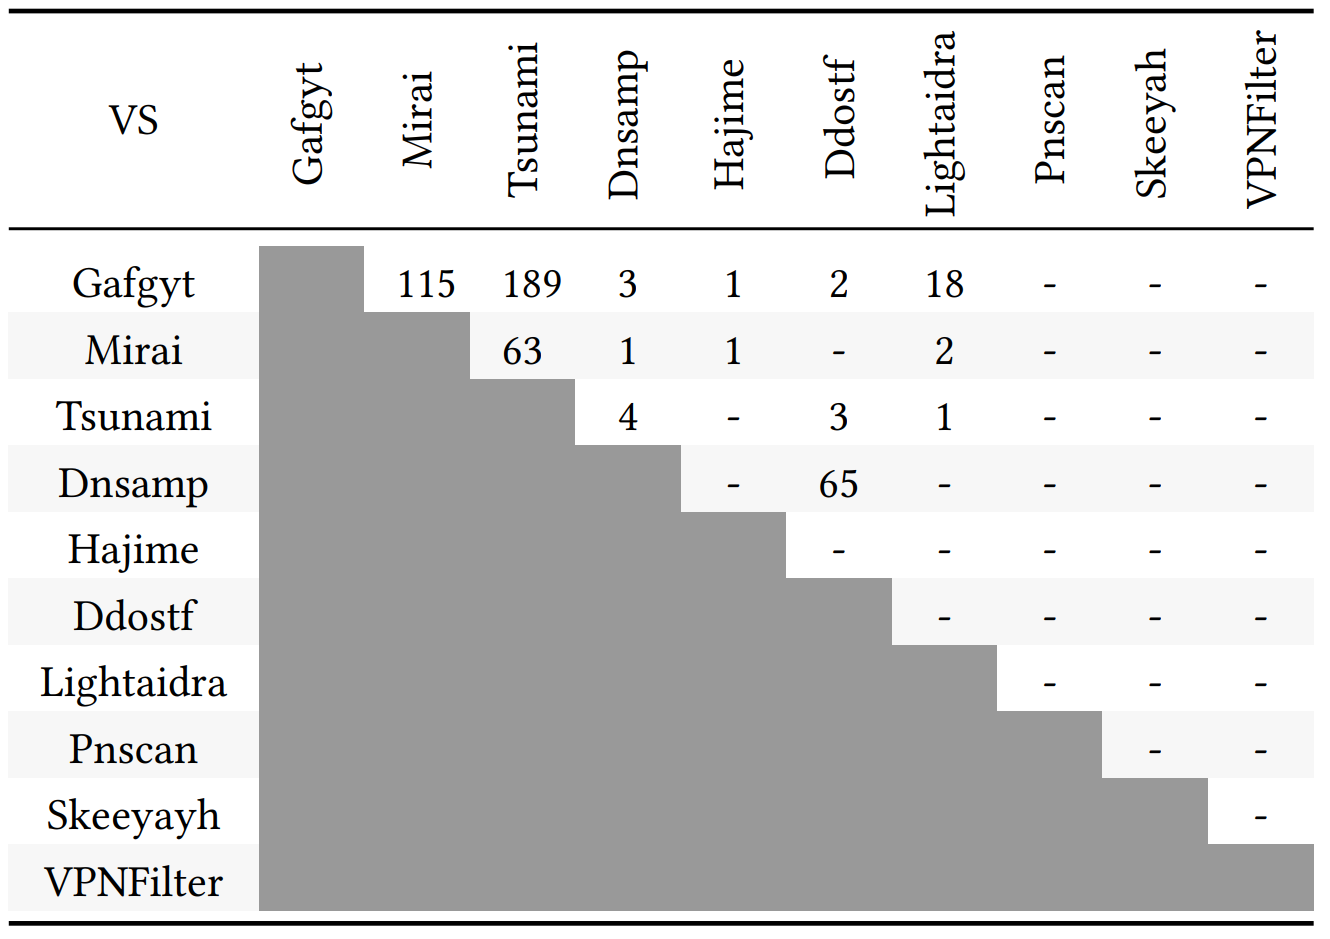
\includegraphics[width=0.7\linewidth]{Images/CodeReuse.png}
    \caption{Common functions across top-10 malware families.}
    \label{fig:CodeReuse}
\end{figure}

\noindent To be able to divide library function from user defined function in stripped malware, Cozzi built a database of symbols extracted from different versions of Glibc and uClibc. He also used the non-stripped binaries to create a database of user defined functions used in IoT malware, and then used Diaphora\footnote{For more information, visit www.diaphora.re}, the most advanced program diffing (\textit{i.e.}, comparing and highlighting the differences between two sets of data) tool, to check if the same functions were used in the stripped binaries. \\
A similar idea may be employed also in our case: a database with sensitive functions (or variants of them) could be created, and then we could analyze the centrality measures of the functions contained in the sample's call graph that, using Diaphora, obtained a high enough similarity score to one of the function inside the database. These function could be both library functions or specific used defined function that are commonly found in malware families. However, an extensive study on what these functions could be is needed before being able to test this idea.

\section{Final Considerations}
Even though malware analysis for IoT is still in its early stages, the threat is growing rapidly. Due to the lack of security of most embedded devices, most malicious programs don't even need to be obscured or packed like most of their Windows counterparts. However it won't take long before proper countermeasures to debugging and analysis are applied also to IoT malware. \\
Many more advanced studies, like Cozzi's \cite{cozzi2020binary}, are needed to be able to fully understand how they work, but, even more important than that, how they evolve. Especially because, nowadays, embedded devices are becoming a bigger and bigger part of our lives, while also often collecting and transmitting sensitive data.